\section{LWMPI: Lightweight MPI for Manycores}
\label{sec:proposal}

	% Present LWMPI
	Aiming at better programmability in lightweight manycores,
	we propose \lwmpi\footnote{\lwmpi is available at:
	\url{https://github.com/nanvix/libmpi}}: an \mpi library for these
	processors.
	%
	% Aims (portability, programmability, cope with restritions)
	The design goals that guided the implementation of \lwmpi are:
	%
	\begin{enumerate}[label=(\roman*)]
		\item \textit{portability}: the library should be portable and
			applicable to various \lws; we enable this by designing it
			on top of a \posix-compliant \os (Nanvix);

		\item \textit{compatibility}: the implementation
			must comply with the \mpi specification; it sticks to the
			3.1 version;

		\item \textit{extendability}: it should be possible to add new
			functions or submodules to the implementation with little
			effort; as so, we design it in a tier-based scheme; and

		\item \textit{lightness}: the implementation should be simple and
			lightweight to cope with restrictive resources of \lws; this way,
			we implemented it from scratch, rather than adapting an existing
			heavy-weight solution like
			% OpenMPI~\cite{OpenMPI2020} or
			% MPICH~\cite{MPICH2020}.
			OpenMPI\footnote{OpenMPI website: \url{https://www.open-mpi.org}} or
			MPICH\footnote{MPICH website: \url{https://www.mpich.org}}
	\end{enumerate}


\subsection{\lwmpi Architecture}
\label{sec:libmpi-impl}

	% Justifying partial support
	Currently, \lwmpi implements an initial subset of the \mpi
	specification (version 3.1). We opted for this partial support since
	fully implementing the entire standard would result in a much bigger
	memory footprint, violating the \textit{lightness} design goal.
	%
	% LWMPI architectural overview
	Figure~\ref{figure:libmpi-arch} presents the two-tier approach
	adopted by \lwmpi on top of \nanvix.

	\begin{figure}[t]
		\centering
		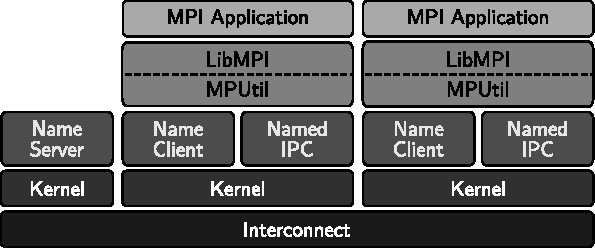
\includegraphics[width=0.9\linewidth]{libmpi}
		\caption{Architectural overview of \lwmpi.}
		\label{figure:libmpi-arch}
		\vspace{-15pt}
	\end{figure}

	The \libmpi tier encapsulates the top-level library and is the
	entry point for user applications.
	%
	% Layer overview
	This layer exposes the library interface and implements the backend
	functions over \mputil. It focuses on filtering
	the input parameters given by the user, performing the
	runtime management and choosing the underlying protocols employed by
	the \mpi calls.
	%
	% Already implemented in LWMPI
	In its current version, our library implements: functions for
	\textit{runtime management}, such as \texttt{MPI\_Init} and
	\texttt{MPI\_Finalize}; support for \textit{communicators} and
	information retrieving, such as \texttt{MPI\_Comm\_rank} and
	\texttt{MPI\_Comm\_size}; support for \textit{groups} of communication
	similarly to communicators;	\textit{error handlers}; and point-to-point
	communication via \mpisend and \mpirecv in the synchronous mode and
	carrying any of the predefined \textit{data types} for the C language.

	% MPUTIL presenting
	The \mputil tier is the middle layer between the overlying library and
	the base \os. Precisely, it is responsible for translating the requests
	from \libmpi to the \nanvix interface. \mputil exposes elementary
	abstractions that support the top-level tier, aiming at keeping the
	library implementation decoupled from the \os interface. It is also
	in this level where the communication protocols used in the \mpi calls
	are implemented.
	%
	% MPUTIL positioning
	To perform these protocols, \mputil relies on the named \ipc
	abstractions exposed by the \textit{Name Service} of the \nanvix
	runtime system, which include
	primitives for fine-grain fixed-size transfers (\mailbox),
	coarse-grain fixed-size transfers (\portal), and
	synchronization points (\sync)~\cite{Souto2020}.

\subsection{Point-to-Point Communication in \lwmpi}
\label{sec:lwbmpi-sendrecv}

	\begin{figure}[b]
		\centering
		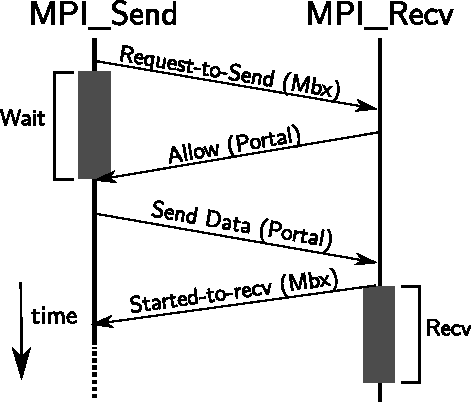
\includegraphics[width=0.55\linewidth]{send-recv_protocol}
		\caption{Communication protocol.}
		\label{figure:comm-protocol}
	\end{figure}

	% Present figures
	Currently, \lwmpi uses the \textit{synchronous mode} to carry out
	communications in \mpisend and \mpirecv functions
	to avoid extra memory usage and keep the library thin (\ie messages
	are not buffered). Figure~\ref{figure:comm-protocol} shows the
	inter-process interaction from the perspective of message exchanges.

	% Send and recv start (steps 1.1 and 2.1)
	Initially, when a \mpisend call is issued, the
	sender builds a request and transfers it to the target process
	through \mailbox, waiting for the receiver to establish the communication.
	The transferred header includes all the information needed by the receiver
	to match a correspondent \mpirecv with the registered request, \ie
	communicator id, tag and source/destination.
	%
	At the receiver side, when a \mpirecv call is issued, it looks for
	incoming requests that arrived or blocks waiting for a matching
	one, if none has been found.

	When a matching request is found, the receiver emits an allow signal
	to the output \portal of the sender, unblocking it and giving permission
	to start the data transfer. The sender, then, starts to send the data
	using the high bandwidth channel. When the receiver starts to receive the
	data in its input \portal, it issues a second started-to-receive signal
	to the sender, signaling that the sender can successfully return when it
	transmitted all the data through the channel, or if it has already done that.
	%
	The receiver will return from \mpirecv when it has
	read all the data from the channel, or have read the amount of data
	equivalent to the local user buffer size.
